\subsection{LZ78}

\begin{frame}{\FrameName}
	\begin{block}{LZ78}
		\begin{itemize}[<+->]
			\item Gänginger Kompressionsalgorithmus
			\item Abraham Lempel \& Jacob Ziv (1978)
			\item Verwendung GIF \& TIFF \PDFC{Erweiterung wird verwendet}
		\end{itemize}
	\end{block}
	\end{frame}

\begin{frame}{\FrameName}
\begin{block}{LZ78 - Datenstrukturen}
	\begin{itemize}[<+->]
		\item Strings $\rightarrow$ Sequenzen von Paaren $(i,c)$ \linebreak \Hint{$i$...Index eines Vorgänger-Paares oder $0$$; c \in \Sigma$}
		\item<3-> Paar $\hat{=}$ Substring
		\item<4-> Wenn $i$ gleich $0$ dann ist dieser Substring gleich $c$
		\item<4-> Andernfalls ist der Substring des $i$-ten Paares gefolgt von $c$
		\item<1->[] \Gap \begin{center}
			\only<1>{
				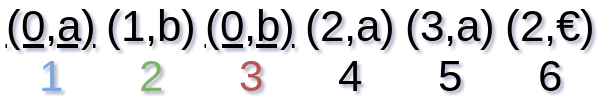
\includegraphics[width=0.6\textwidth]{Images/LZ78/blank}}
			\only<2-4>{
				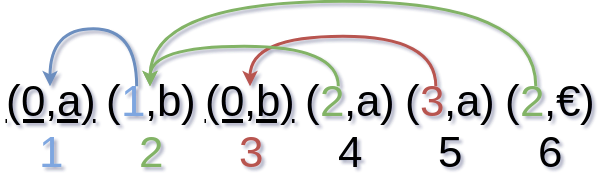
\includegraphics[width=0.6\textwidth]{Images/LZ78/withRefs}}
			\only<5>{
				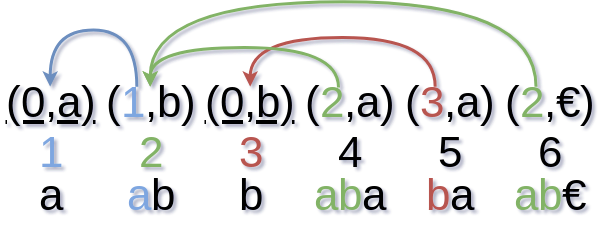
\includegraphics[width=0.6\textwidth]{Images/LZ78/full}}
		\end{center}
	\end{itemize}
\end{block}
\end{frame}

\begin{frame}{\FrameName}
	\begin{block}{LZ78 - Grammatiken}
		\begin{itemize}[<+->]
			\item Paar $\hat{=}$ Nichterminal
			\item $\begin{cases}
				X_j \rightarrow c, & i = 0\\
				X_j \rightarrow X_i c, & \text{sonst}
			\end{cases}$
			\item $S \rightarrow X_1 ... X_k$
			
		\end{itemize}
		\visible<4>{
			\begin{minipage}[t]{0.5\textwidth}
				$S \rightarrow \foreach \n in {1,2,3,4,5,6}{X_{\n}}$ 
				
	
				$X_1 \rightarrow a; X_2 \rightarrow X_1b;  X_3 \rightarrow b$
				$X_4 \rightarrow X_2a; X_5 \rightarrow X_3a; X_4 \rightarrow X_6\text{\euro}$
			\end{minipage}
			\begin{minipage}[c]{0.48\textwidth}
				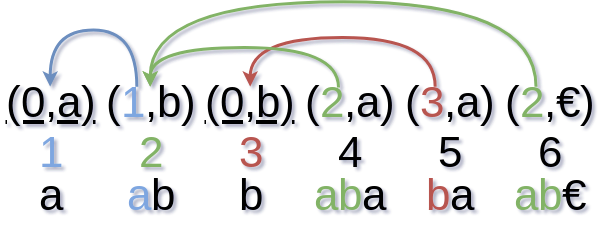
\includegraphics[width=\textwidth]{Images/LZ78/full}
			\end{minipage}
		}
	
	\end{block}
	\end{frame}

\begin{frame}{\FrameName}
\begin{block}{LZ78 - Algorithmus}
	\begin{itemize}[<+->]
		\item String sequenziell (von links nach rechts) übersetzt
		\item Iteration: finde kürzestes Präfix $\gamma$ des in Strings das nicht Expansion eines bereits erzeugten Paars ist
		% \item Am Ende des Strings muss eventuell ein weiteres Zeichen hinzugefügt werden
		\item Übersetzungsvorschrift:
		\begin{enumerate}
			\item<4-> Wenn $|\gamma| = 1$ $\Rightarrow$ $(0,\gamma)$
			\item<5-> Andernfalls ist $\gamma = \alpha c$. \linebreak $\alpha$ ... Expansion eines Paars mit dem Index $i_\alpha$ \linebreak $\Rightarrow$ Paar: $(i,c)$
		\end{enumerate}
	\end{itemize}
\end{block}
\end{frame}

% Marking string sequence
\newcommand{\M}[1]{\textcolor{OrangeRed}{#1}}

\begin{frame}{\FrameName}
\begin{block}{Beispiel}
	\begin{description}[<+->]
		\item \M{a}abbababaab\euro
		\item $\underbrace{(0,a)}_{a}$ \M{ab}bababaab\euro
		\item $\underbrace{(0,a)}_{a}$ $\underbrace{(1,b)}_{ab}$ \M{b}ababaab\euro
		\item $\underbrace{(0,a)}_{a}$ $\underbrace{(1,b)}_{ab}$ $\underbrace{(0,b)}_{b}$ \M{aba}baab\euro
		\item $\underbrace{(0,a)}_{a}$ $\underbrace{(1,b)}_{ab}$ $\underbrace{(0,b)}_{b}$ $\underbrace{(2,a)}_{aba}$ \M{ba}ab\euro
		\item $\underbrace{(0,a)}_{a}$ $\underbrace{(1,b)}_{ab}$ $\underbrace{(0,b)}_{b}$ $\underbrace{(2,a)}_{aba}$ $\underbrace{(3,a)}_{ba}$ \M{ab\euro}
		\item $\underbrace{(0,a)}_{a}$ $\underbrace{(1,b)}_{ab}$ $\underbrace{(0,b)}_{b}$ $\underbrace{(2,a)}_{aba}$ $\underbrace{(3,a)}_{ba}$ $\underbrace{(2,\text{\euro})}_{ab\text{\euro}}$
	\end{description}
\end{block}
\end{frame}

\begin{frame}{\FrameName}
	\begin{block}{Lower Bound}
		\begin{itemize}[<+->]
			\item Definiere $\alpha_k$ \textcolor{gray}{(n = $|\alpha_k |$)} \PDFC{alpha wächst dynamisch}
			\item Bestimme upper bound von $m^*$ \linebreak \textcolor{gray}{$m^* \in \mathcal{O}(\UpperBound)$}
			\item Bestimme lower bound von $m$ \linebreak \textcolor{gray}{$m \in \Omega(\LowerBound)$}
			\item[$\Rightarrow$] \fbox{
			$a(n) \in \Omega(\frac{
				\LowerBound
			}{
				\UpperBound
			})$
			}
		\end{itemize}
	\end{block}
	\end{frame}

\newcommand{\StringDefinition}{$$ \alpha_k = a^1 a^2 ... a^k \underbrace{ba^k...ba^k}_{(k+1)^2}$$ $$ \alpha_k = a^{k(k+1)/2}(ba^k)^{(k+1)^2} $$}

\begin{frame}{\FrameName}
\begin{block}{Lower Bound (1/4)}
	$$ \alpha_k = a^1 a^2 ... a^k \underbrace{ba^k...ba^k}_{(k+1)^2}$$
	\visible<2->{$$ \alpha_k = a^{k(k+1)/2}(ba^k)^{(k+1)^2} $$}
	\begin{itemize}[<+->]
		\item<3-> \only<3>{$|\alpha_k | = k \frac{k+1}{2} + (1+k)(k+1)^2$} \only<4->{$|\alpha_k | = \alert<5>{k^3} + \frac{7}{2}k^2 + \frac{7}{2}k + 1$}
		\item<5-> $ n = |\alpha_k | \in \Theta(\alert{k^3})$
	\end{itemize}
\end{block}
\end{frame}

\begin{frame}{\FrameName}
\begin{block}{Lower Bound (2/4)}
	\StringDefinition
	\begin{itemize}[<+->]
		\item Es existiert Grammatik mit Größe: \Hint{(Lemmma 1...3)} $\mathcal{O}(\underbrace{1+ log(\frac{k^2+k}{2})}_{a^{k(k+1)/2}} + \underbrace{log((k+1)^2) + 1+ 1+ log(k)}_{(ba^k)^{(k+1)^2}})$
		\item \only<2>{$m^* \in \mathcal{O}(1+ log(\frac{k^2+k}{2}) + log((k+1)^2) + 1+ 1+  log(k))$} 
			\only<3>{$m^* \in \mathcal{O}(log(\frac{k^2+k}{2}) + log((k+1)^2) + log(k))$}
			\only<4>{$m^* \in \mathcal{O}(2log(k) + 2log(k) + log(k))$}
			\only<5->{$m^* \in \mathcal{O}(log(k))$}

		\item<6-> $m^* \in \mathcal{O}(log(n^\frac{1}{3}))$ \Hint{$ n \in \Theta(k^3)$}
		\item<7-> $m^* \in \mathcal{O}(log(n))$
	\end{itemize}
\end{block}
\end{frame}

\begin{frame}{\FrameName}
\begin{block}{Lower Bound (3/4)}
	\StringDefinition
	\begin{itemize}[<+->]
		\item String wird in zwei Phasen in eine Paar-Sequenz übersetzt
		\item Erste Phase: alle Strings $a...a^k$ zu Paaren übersetzt
		\item Zweite Phase: $a^iba^j$ für alle $i,j \in [0,k]$ wird ein Paar erstellt
		\item $m \in \Omega(\sum_{z=1}^k z + (k+1)^2) = \Omega(k^2)$
		\item $m \in \Omega(n^{2/3})$
	\end{itemize}
\end{block}
\end{frame}

\begin{frame}{\FrameName}
\begin{block}{Lower Bound (4/4)}
	\StringDefinition	
		$m^* \in \mathcal{O}(log \thinspace n)$ \hfill $m \in \Omega(n^{2/3})$ \linebreak 
		\begin{center}
			\visible<2>{$a(n) \in \Omega(\frac{n^{2/3}}{log \thinspace n})$}
		\end{center}
\end{block}
\end{frame}

\begin{frame}{\FrameName}
	\begin{block}{Upper bound}
		\begin{itemize}[<+->]
			\item $m$ proportional zu zu Anzahl der Nichterminale
			\item Nichterminale in Gruppen zerlegt
			\item Abhängigkeit Anzahl Nichterminal und Anzahl Gruppen
			\item Abschätzung der Gruppenanzahl
			\item $m$ bestimmen
		\end{itemize}
	\end{block}
	\end{frame}



\begin{frame}{\FrameName}
	\begin{block}{Upper bound (1/4)}
		\visible<1->{
			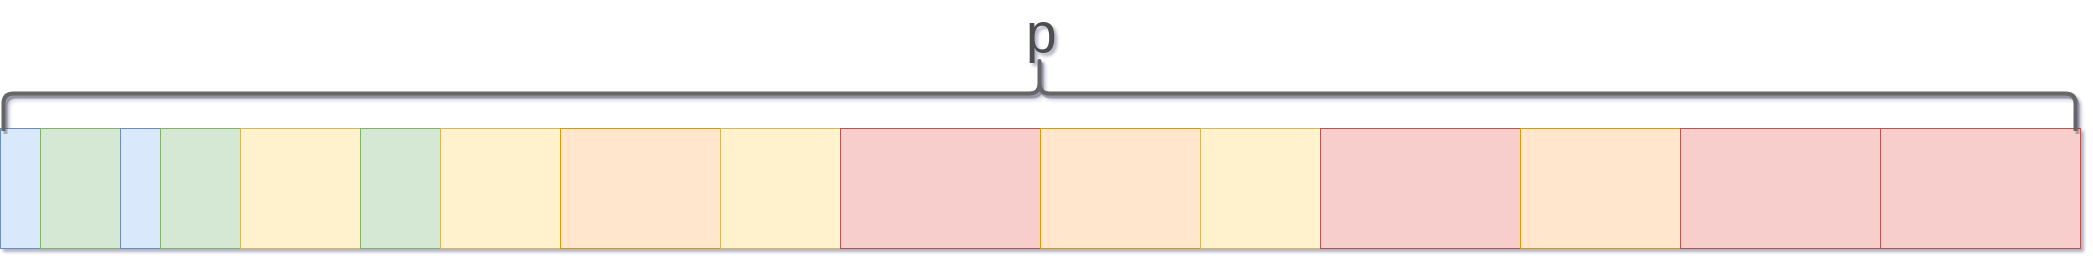
\includegraphics[width=0.98\textwidth]{Images/LZ78/UB_unsort}}
			\Gap
		\visible<2->{
			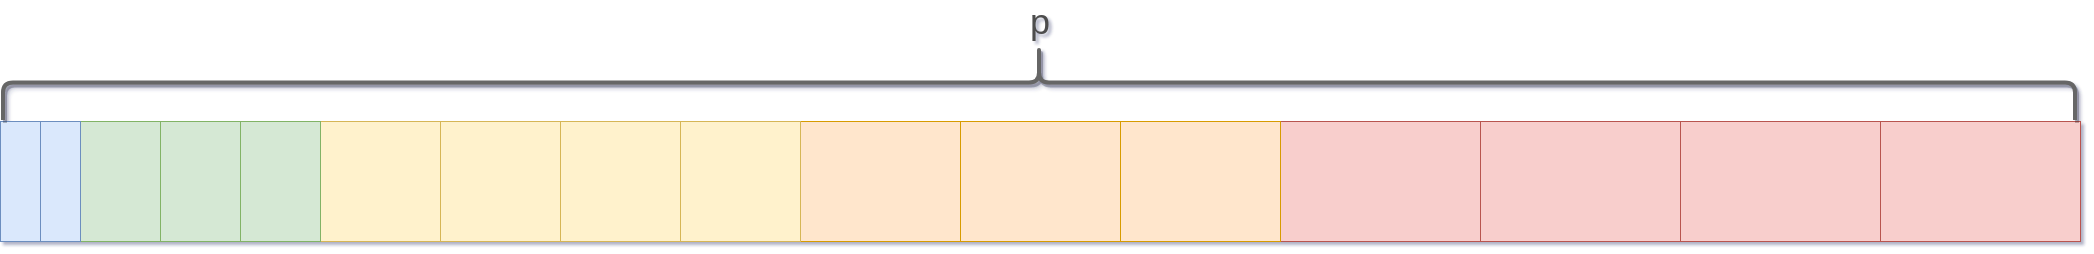
\includegraphics[width=0.98\textwidth]{Images/LZ78/UB_sort}}
			\Gap
		\visible<3->{
			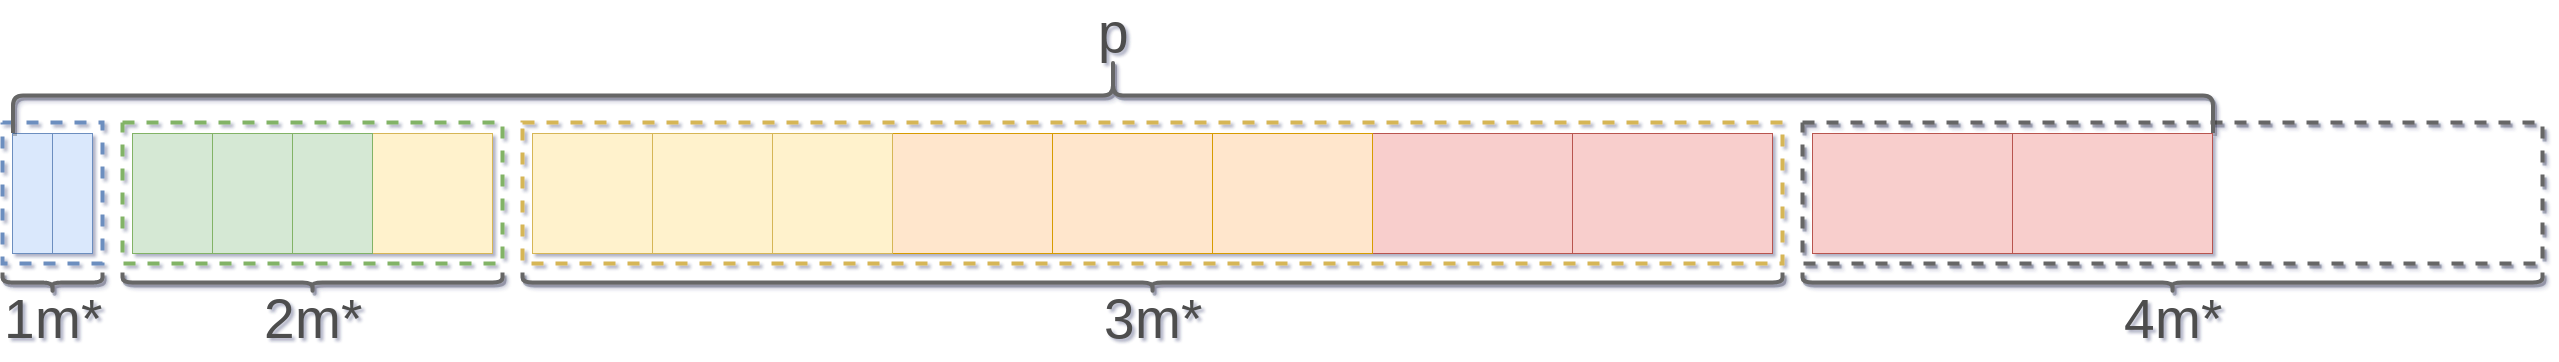
\includegraphics[width=0.98\textwidth]{Images/LZ78/UB_grouped}}
	\end{block}
	\end{frame}

